\section{It lives!}

OntoBG, by what this works propose, is defined and explained here. Following the directives and scope it does not cover the whole of possibilities. It aims to provide new insight on boardgame modeling and study. 

The ontology is composed of four diagrams. A more general which express the MDA behaviour throughout the ontology. Three others which relay the understanding of each part of the MDA, that is, representing OntoBG-M, OntoBG-D and OntoBG-A. Following each of them is presented and explained in a section. Exposing how they came to be, their meaning and how to use each for your own purposes.  

\subsection{The beginning}

Translating the MDA framework into UFO led to a simple diagram with important information. Although simplistic MDA has a lot of nuances. When addressed in a more complex language this nuances need careful analysis to be correctly modeled. The diagram features in \autoref{fig:gamediagram} and its information detailed in sequence.

\begin{figure}[!h]
    \centering
    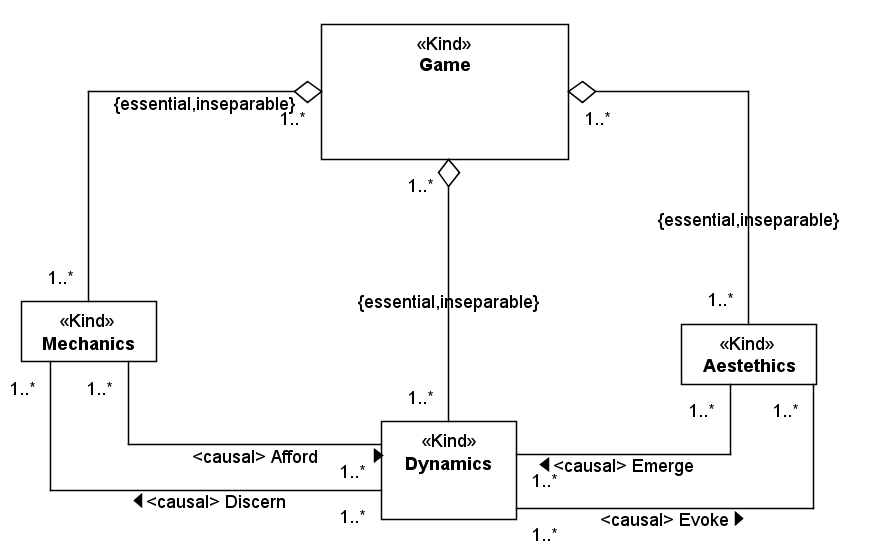
\includegraphics[scale=0.65]{Images/Model/Game.png}
    \caption{Game Diagram}
    \label{fig:gamediagram}
\end{figure}

